\section{The foosball robot system}\label{sec:system}
A simple diagramm of the final system is shown in the figure~\ref{fig:system}.
The system consists of a camera below the table, to monitor the game.
The camera is connected to a PC, which processes the images and sends the commands to the controller unit.
The controller unit moves the motors to the desired position.
% create a simple drawing of the system
\begin{center}
    \begin{figure}[H]
        \centering
        \begin{tikzpicture}
            \draw[fill=green!5] (7, 10) rectangle (0, 0);
            \begin{scope}
                [shift={(3.5, 0)}]
                \node[below] {Foosball table};
            \end{scope}
%        draw a circle in the middle and an arrow pointing there labling it the camera
            \draw[fill=blue!30] (3.5, 5) circle (0.5) node[below, yshift=-0.5cm] {Camera below table};
%        \draw[<-] (4.1, 5) -- (8, 5) node[above] {Camera};
%            pc
            \draw[fill=orange!30] (10, 9) rectangle (12, 11) node[pos=0.5] {PC};
%            cable from camera to pc
            \draw[->, blue] (3.5, 5.5) -- (3.5, 6) -- (11, 6) -- (11, 8.8);
%            controler (Arduino)
            \draw[fill=orange!30] (6, 10) rectangle (9, 11) node[pos=.5]{Controller unit};
            \draw[->, blue] (10, 10.5) -- (9.2, 10.5);
%            move motor
            \draw[fill=blue!30] (7, 6.5) rectangle (8.5, 8) node[pos=.5,
            text width=1.5cm,align=center
            ] {Move motor};
            \begin{scope}
                [shift={(7.75, 7.25)}, scale=0.4]
                \draw \gear{18}{2}{2.4}{10}{2};
            \end{scope}
            \draw[fill, black] (7.75, 7.25) circle (0.03);
            \draw[<-, blue](7.75, 8.2) -- (7.75, 10);
%        tube
            \draw[fill=black!20] (0, 8.75) rectangle (9, 8.25) node[pos=.5, shift={(1, 0)}] {Tube};
            \draw[fill=blue!30] (0, 9.25) rectangle (-1, 7.75) node[midway, left, shift={(-.5, 0)}] {Shoot motor};
            \draw[->, blue] (6, 10.5) -- (-0.5, 10.5) -- (-0.5, 9.45);
            \draw[fill=red] (3.5, 8.5) circle (0.5) node[below, yshift=-0.5cm] {Goalkeeper};
        \end{tikzpicture}
        \caption{The foosball robot system}
        \label{fig:system}
    \end{figure}
\end{center}

\newpage
\section{Motors}\label{sec:motors}
The motors have two primary tasks: positioning the goalkeeper and shooting the ball.
A stepper motor controls the goalkeeper's movement, while a DC motor powers the ball's acceleration.
The goalkeeper must defend against balls traveling at a maximum velocity of $v_{max}=7\text{m/s}$.
To meet this requirement, calculations are necessary to determine the required torque and speed for each motor.

\subsection{Table measurements}\label{subsec:table_measurements}
Accurate foosball table measurements are essential for calculating the motors' torque and speed.
Figure~\ref{fig:table_measurements} illustrates these measurements:
\begin{itemize}
    \item The ball travels $400\text{mm}$ from the attacker to the goal.
    \item The goalkeeper moves a distance of $180\text{mm}$.
    \item The whole table is $700\text{mm}$ wide.
\end{itemize}

\begin{center}
    \begin{figure}[H]
        \centering
        \begin{tikzpicture}
            \node[anchor=south west,inner sep=0] (image) at (0,0) {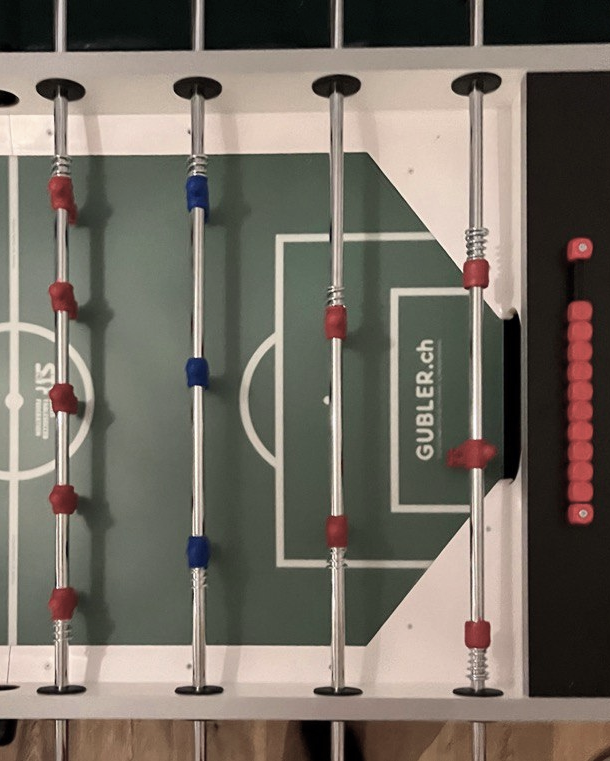
\includegraphics[width=0.5\textwidth, opacity=0.8]{../photos/foosball_table}};
            \begin{scope}
                [x={(image.south east)},y={(image.north west)}]
%        \draw[help lines,xstep=.1,ystep=.1] (0,0) grid (1,1);
%        \foreach \x in {0,1,...,9} { \node [anchor=north] at (\x/10,0) {0.\x}; }
%        \foreach \y in {0,1,...,9} { \node [anchor=east] at (0,\y/10) {0.\y}; }
                \def \tubex {0.76};
%        \draw[red,ultra thick,rounded corners] (0.62,0.65) rectangle (0.78,0.75);
                \draw[<->,white,rounded corners, line width=1.5mm] (\tubex, 0.9)  -- (\tubex, 0.65) node[midway, left, fill=black, fill opacity=0.8,text opacity=1,rounded corners=2pt,inner sep=1pt] {\huge \textbf{180mm}};
                \draw[<->,white,rounded corners, line width=1.5mm] (0.85, 0.9)  -- (0.85, 0.09) node[pos=0.85, left, fill=black, fill opacity=0.8,text opacity=1,rounded corners=2pt,inner sep=1pt] {\huge \textbf{700mm}};
                \draw[<->,white,rounded corners, line width=1.5mm] (0.335, 0.5)  -- (0.775, 0.5) node[pos=0.85, left, fill=black, fill opacity=0.8,text opacity=1,rounded corners=2pt,inner sep=1pt] {\huge \textbf{400mm}};

            \end{scope}
        \end{tikzpicture}
        \caption{Foosball table with measurements}
        \label{fig:table_measurements}
    \end{figure}
\end{center}
%\todo{The calculations dont make completly sense, i think i made a mistake somewhere and bought an overpowered motor, which is fine i guess}

\subsection{Calculations for the moving motor}\label{subsec:moving_motor}
The distance from the foremost attacker to the goal is $s=0.4m$.
That means the player has to stop the ball in time $t_s$, where
\begin{equation}
    \label{eq:stopping_time}
    t_s = \frac{s}{v} = \frac{0.4m}{7m/s} \approx 0.057 s.
\end{equation}
This is not a lot of time to process the image and move the motors.
I round the travel distance of the goalkeeper from $180mm$ to $200mm$ for the calculations because there is a spring at either end which can be compressed.
I always keep the goalkeeper in the middle, such that the player has to travel a maximum distance of $0.1m$.
That means the player has an average velocity of
\begin{equation}
    \label{eq:average_velocity}
    \bar{v} = \frac{s}{t_s} = \frac{0.1m}{0.057s} \approx 1.75m/s.
\end{equation}
I assume a constant acceleration and deceleration, so when the player reaches the top speed it needs to decelerate immediately, to keep the forces as low as possible.
A graph to explain the velocity can be seen here:

\begin{center}
    \begin{tikzpicture}
        \centering
        \begin{axis}
            [
            axis x line=center,
            axis y line=center,
            width={0.2\linewidth},
            xtick=none,
            ytick={0,1},
            yticklabels={,$v_{max}$},
            xlabel={$t$},
            ylabel={$v$},
            xlabel style={below right},
            ylabel style={above left},
            xmin=-0.2,
            xmax=2.2,
            ymin=-0.2,
            ymax=1.2]

            \addplot [] table {
                0 0
                1 1
                2 0
            };
        \end{axis}
    \end{tikzpicture}
\end{center}

\noindent Which means the player has a top speed of $v_{max}=2\cdot1.75m/s=3.5m/s$.
The motor also needs to be able to accelerate the player in $0.057s/2=0.0285s$, which means the motor needs to be able to achieve a maximum acceleration $a_{max}$ of
\begin{equation}
    \label{eq:acceleration}
    a_{max} = \frac{v_{max}}{t_s} = \frac{3.5m/s}{0.0285s} = 122.8m/s^2.
\end{equation}
I assume that the weight of the tubes is $m \approx 0.1kg$.
The torque needed to move the tubes is
\begin{equation}
    \label{eq:torque}
    \tau = F \cdot r = m \cdot a \cdot r = 0.1kg \cdot 122.8m/s^2 \cdot 0.083m \approx 1Nm
\end{equation}
assuming the radius $r_g$ of the gear is 8.3cm and the required top rotational speed (measured in rotations per minute (RPM)) is
\begin{equation}
    \label{eq:top_rpm}
    \frac{v}{2\pi r_g} \cdot 60s/min = \frac{7m/s}{2\pi \cdot 0.083m} \cdot 60s/min \approx 800\text{RPM}.
\end{equation}
A motor that fits those requirements is the \textbf{PD42-3-1141\autocite{PD42-3-1141}} from \textbf{Trinamic}.

\subsection{Calculations for the shooting motor}\label{subsec:rotating_motor}
The ball has a mass $m_{ball}=17g$.
I assume that I have an angle of $45\deg$ ($=\frac{\pi}{4}$ in radians) to accelerate the ball.
\\
\begin{center}

    \tikzset{
        testpic/.pic={
            \node at (0.05,-0.35) {
\includegraphics[height=3.2cm] {../photos/foosball_player}};
        },
        testpic2/.pic={
            \node at (0.05,-0.35) {
\includegraphics[height=3.2cm] {../photos/foosball_player}};
        },
    }

    \begin{tikzpicture}
        \def \r {2cm}
        \def \rsmall {0.5}
        \def \angle {45}
        \pic[rotate=45/2,transform shape] at (0,0) {testpic};
        \pic[rotate=-45/2,transform shape] at (0,0) {testpic2};
        \draw (0,0) -- ({-sin(\angle / 2)*\r}, {-cos(\angle / 2)*\r});
        \draw (0,0) -- ({sin(\angle / 2)*\r}, {-cos(\angle / 2)*\r}) node[right, midway] {$r_p=70\text{mm}$};
        \draw ({-sin(\angle / 2)*\rsmall}, {-cos(\angle / 2)*\rsmall}) arc(270-\angle/2:270+\angle/2:\rsmall) node[midway,below] {$45\deg$};
        \draw[->] ({-sin(\angle / 2)*\r}, {-cos(\angle / 2)*\r}) arc(270-\angle/2:270+\angle/2:\r) node[midway,below] {$l$};
%        \draw () circle (\r);
    \end{tikzpicture}
\end{center}
%    \\
That means the player has the distance $l$ (arc length) to accelerate the ball together with the player.
\begin{equation}
    \label{eq:arc-length}
    l = r_p \cdot \frac{\pi}{4} = 70mm \cdot \frac{\pi}{4} = 55mm
\end{equation}
The goal is to shoot the ball back at a speed of $7m/s$.
The time to make one full rotation with the given speed of $v_{max}=7m/s$ is
\begin{equation}
    \label{eq:time-rot}
    t_{rot} = \frac{2\pi\cdot r_p}{v_{max}} = \frac{2\pi\cdot 70mm}{7m/s} = \frac{\pi}{50} \approx 0.06s
\end{equation}
The maximum speed can easily be calculated with
\begin{equation}
    \label{eq:max_speed}
    \omega = \frac{60s/min}{t_{rot}} = \frac{60s/min}{0.06s/rotation} = 1000\text{RPM}
\end{equation}
%\todo{Compute the torque needed to accelerate the ball}
To calculate the torque needed to accelerate the ball, I need to know the time it takes to accelerate the ball to full speed.
This can be done by integrating the acceleration twice over time and solving for the time.
The integration constants can be discarded because the distance and velocity are zero at the beginning.
\begin{equation}
    \label{eq:time_to_full_speed}
    v = \int a \cdot dt = a \cdot t \Rightarrow t=\frac{v}{a}
\end{equation}
The length $l$ and the acceleration $a$ can be calculated by using the double integral of the acceleration over time.
\begin{equation}
    \label{eq:shoot_acceleration}
    l = \int v \cdot dt = \int a \cdot t \cdot dt = \frac{1}{2} \cdot a \cdot t^2 \Rightarrow a = \frac{2 \cdot l}{t^2}
\end{equation}
Substituting the time from the equation~\ref{eq:time_to_full_speed} into the equation~\ref{eq:shoot_acceleration} gives the acceleration.
\begin{equation}
    \label{eq:shoot_acceleration_substituted}
    a = \frac{2 \cdot l}{(\frac{v_{max}}{a})^2} = \frac{2 \cdot l \cdot a^2}{v_{max}^2} \Rightarrow a = \frac{v_{max}^2}{2 \cdot l}
\end{equation}
Together with the mass $m_{ball}$ of the ball, the torque needed to accelerate the ball can be calculated.

\begin{equation}
    \label{eq:torque_shoot}
    |\vec{\tau}| = |\vec{r} \times \vec{F}| \xRightarrow{\vec{r} \perp \vec{F}} \tau = F \cdot r_p = m_{ball} \cdot a \cdot r_p = m_{ball} \cdot \frac{v_{max}^2}{2 \cdot l} \cdot r_p
\end{equation}
Together with the length $l$ from equation~\ref{eq:arc-length}, the torque needed to accelerate the ball can be calculated.
\begin{equation}
    \label{eq:torque_shoot_substituted}
    \tau = r_p \cdot m_{ball} \cdot \frac{v_{max}^2}{2\cdot\frac{\pi}{4}\cdot r_p} = 2m_{ball} \cdot \frac{v_{max}^2}{\pi} \approx 0.5Nm
\end{equation}



For the motor that just rotates the player I can use a DC motor with gears and an encoder, as they often have more power and can go faster with less torque and accuracy.
% Pololu 10:1 Metal Gearmotor 37Dx65L mm 12V with 64 CPR Encoder (Helical Pinion) 4758
A motor that fits these requirements is the \textbf{Pololu 10:1 Metal Gearmotor 37Dx65L mm 12V with 64 CPR Encoder (Helical Pinion) 4758}\autocite{pololu-dc}.
Later I realized a made a mistake by not including the moment of inertia of the player.
Including the moment of inertia the equation is a little bit different:
The torque is defined as
\begin{equation}
    \label{eq:torque2}
    \tau = I \frac{d\omega}{dt},
\end{equation}
where $I$ is the moment of inertia and $\omega$ is the angular velocity.
The angular velocity $\omega$ depends linearly on time $t$:
\begin{equation}
    \label{eq:angular_velocity}
    \omega(t) = a_\omega \cdot t
\end{equation}
where $a_\omega$ is the angular acceleration.
Integrating this formula yields a function $\theta(t)$ for the angle $\theta$:
\begin{equation}
    \label{eq:angle}
    \theta(t) = \int \omega(t)dt = \int a_\omega \cdot t dt = \frac{1}{2} a_\omega t^2
\end{equation}
At time $t_e$, the player has rotated by $45\deg = \frac{\pi}{4}$.
Substituting $t_e$ into the equation~\ref{eq:angle} and solving for $t_e$:
\begin{equation}
    \label{eq:time_to_rotate}
   \theta(t_e)= \frac{1}{2} a_\omega t_e^2 = \frac{\pi}{4} \Rightarrow t_e = \sqrt{\frac{\pi}{2a_\omega}}
\end{equation}
Substituting $t_e$ into the equation~\ref{eq:angular_velocity} and knowing that the player has an angular velocity $\omega_e=\frac{2\pi}{t_{rot}}$, gives an equation for the angular acceleration, which can be solved for the angular acceleration $a_\omega$:
\begin{equation}
    \label{eq:angular_acceleration}
    \omega(t_e) = \omega_e = \frac{2\pi}{t_{rot}} \Rightarrow a_{\omega} \cdot \sqrt {\frac{\pi}{2a_{\omega}}} = \frac{2\pi}{t_{rot}} \Rightarrow a_{\omega} = \frac{8\pi}{t_{rot}^2}
\end{equation}
Therefore the function $\omega(t)$ is:
\begin{equation}
    \label{eq:angular_velocity_function}
    \omega(t) = \frac{8\pi}{t_{rot}^2} \cdot t
\end{equation}
And the required torque $\tau$ is:
\begin{equation}
    \label{eq:torque3}
    \tau = I_s \frac{d\vec{\omega}}{dt} = I \frac{8\pi}{t_{rot}^2}
\end{equation}
I approximate the player with a tube and the axis going through it at the distance $s=\frac{l}{6}$ from the center axis.
The moment of inertia of a tube is:
\begin{equation}
    \label{eq:moment_of_inertia}
    I = \frac{1}{12} m_{player} \cdot l^2
\end{equation}
To shift the axis of rotation, the Parallel axis theorem can be used:
\begin{equation}
    \label{eq:parallel_axis_theorem}
    I_0 = I_{S} + m_{player} \cdot s^2
\end{equation}
where $I_0$ is the moment of inertia around the shifted axis, $I_{S}$ is the moment of inertia around the center axis and $s$ is the distance from the center axis to the shifted axis.
Therefore, the moment of inertia $I_0$ is:
\begin{equation}
    \label{eq:moment_of_inertia_shifted}
    I_0 = \frac{1}{12} m_{player} \cdot l^2 + m_{player} \cdot s^2 = \frac{1}{12} m_{player} \cdot l^2 + m_{player} \cdot \left(\frac{l}{6}\right)^2 = \frac{1}{12} m_{player} \cdot l^2 + \frac{1}{36} m_{player} \cdot l^2 = \frac{1}{9} m_{player} \cdot l^2
\end{equation}
Substituting the moment of inertia $I_0$, $l=\frac{3}{2}r_p$ and $m_{player}=50g$ into the equation~\ref{eq:torque3} gives the torque needed to accelerate the player:
\begin{equation}
    \label{eq:torque4}
    \begin{split}
        \tau &= \frac{8\pi}{t_{rot}^2} \cdot \frac{1}{9} m_{player} \cdot l^2 = \frac{8\pi}{t_{rot}^2} \cdot \frac{1}{9} m_{player} \cdot \left(\frac{3}{2}r_p\right)^2\\
        &= \frac{8}{9}m_{player}\pi\frac{\frac{9}{4}r_p^2}{t_{rot}^2}=2m_{player}\pi\frac{r_p^2}{t_{rot}^2}
    \end{split}
\end{equation}
Substituting $t_{rot}$ from equation~\ref{eq:time-rot} yields:
\begin{equation}
    \label{eq:torque5}
    \tau = 2m_{player}\pi\frac{r_p^2\cdot v_{max}^2}{2^{2} \cdot \pi^{2} \cdot r_p^2} = m_{player}\frac{v_{max}^2}{\pi} \approx 0.39Nm
\end{equation}
Adding this to the torque needed to accelerate the ball gives a total torque of $\tau_{total} \approx 0.89Nm$.
So the motor, having a maximum torque $\sim0.5Nm$, is actually not capable of accelerating the player and the ball at the same time, therefore, $v_{max}$ of $7m/s$ cannot be reached.
The calculations to determine the actual $v_{max}$ are left as an exercise to the reader.


\section{Camera}\label{sec:camera}

\subsection{Optics}\label{subsec:lens}
To achieve my goal of defending against balls at speed of up to $7m/s$, I need a camera that can capture the entire table at a framerate of at least 150fps.
I record the table from the bottom to avoid seeing the players and the rods instead of the ball; therefore, I have to replace the floor of the table with a glass plate.
A sensor that achieves this is the \textbf{IMX287 CMOS} sensor from \textbf{Sony}.
This sensor has a width of $w=4.98\text{mm}$.
A schematic of the approximate setup for the camera is shown in the figure~\ref{fig:camera_setup}.\\
\begin{center}
    \begin{figure}[H]
        \centering
        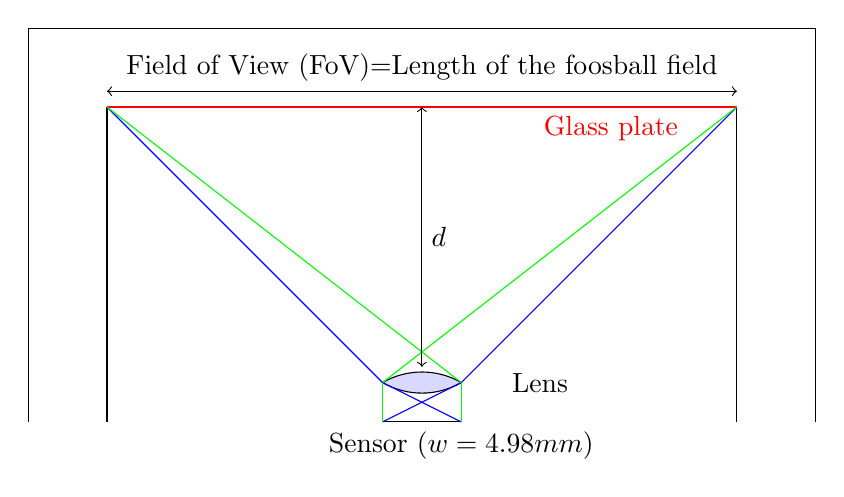
\begin{tikzpicture}
            \draw (0,0) -- (0, 5);
            \draw (0, 5) -- (10, 5);
            \draw (10, 5) -- (10, 0);

            \draw (1,0) -- (1, 4);
            \draw[red] (1, 4) -- (9, 4) node[pos=0.8, below] {Glass plate};
            \draw (9, 4) -- (9, 0);

            \draw (4.5, 0) -- (5.5, 0) node[below] {Sensor ($w=4.98\text{mm}$)};

            \pgfmathsetmacro{\lensRadius}{1}
            \pgfmathsetmacro{\lensHeight}{0.5}
            \pgfmathsetmacro{\startAngle}{asin(\lensHeight/\lensRadius)}

            \draw [fill=blue!15]  (4.5,\lensHeight)
            arc[start angle=180-\startAngle+90,delta angle=2*\startAngle,radius=\lensRadius]
            arc[start angle=-\startAngle+90,delta angle=2*\startAngle,radius=\lensRadius]
            -- cycle; % to get a better line end

            \draw[blue] (1, 4) -- (4.5, \lensHeight);
            \draw[blue] (4.5, \lensHeight) -- (5.5, 0);

            \draw[blue] (9, 4) -- (5.5, \lensHeight);
            \draw[blue] (5.5, \lensHeight) -- (4.5, 0);

            \draw[green] (1, 4) -- (5.5, \lensHeight);
            \draw[green] (5.5, \lensHeight) -- (5.5, 0);

            \draw[green] (9, 4) -- (4.5, \lensHeight);
            \draw[green] (4.5, \lensHeight) -- (4.5, 0);

            \draw (6.5, 0.5) node[]{Lens};
            \draw[<->] (5, 0.70) -- (5, 4) node[midway, right] {$d$};
            \draw[<->] (1, 4.2) -- (9, 4.2) node[above, midway] {Field of View (FoV)=Length of the foosball field};
        \end{tikzpicture}
        \caption{Camera setup}
        \label{fig:camera_setup}
    \end{figure}
\end{center}

\paragraph{Lens Equation}\label{par:lens_equation}

The relationship between the field of view (FoV), the focal length $f$, the sensor width $w$, and the distance to the object $d$ is given by:
\begin{equation}
    \text{FoV} = w \cdot \frac{\text{d}}{f}\label{eq:lens_equation}
\end{equation}


\noindent In my case $d = 700mm$ and my Field of View is $1200mm$ as this is the length of the foosball field.
Now I solve for the focal length $f$:
\begin{equation}
    \label{eq:focal_length}
    f = \frac{w \cdot d}{\text{FoV}} = \frac{4.98\text{mm} \times 700\text{mm}}{1200\text{mm}} \approx 2.9\text{mm}
\end{equation}
% Arducam 2.8-12mm Varifocal C-Mount Lens for Raspberry Pi HQ Camera, with C-CS Adapter
A lens that satisfies these requirements is the \textbf{Arducam 2.8-12mm Varifocal C-Mount Lens for Raspberry Pi HQ Camera, with C-CS Adapter\autocite{arducam-lens}} with a focal length of $2.8-12mm$.
A fitting camera for this lens is the \textbf{Alvium 1800 U-040 with Sony IMX287}\autocite{allied-vision-lens} camera.
Figure~\ref{fig:glass_table} showing the table with the glass plate can be found in the appendix~\ref{sec:images}